\usetikzlibrary{calc}
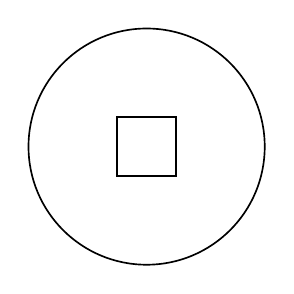
\begin{tikzpicture}[x=1cm,y=1cm,line width=.6pt,font=\normalsize]
\coordinate (O) at (0,0);
\coordinate (Q1) at (-0.375,-0.375);
\coordinate (Q2) at (0.375,-0.375);
\coordinate (Q3) at (0.375,0.375);
\coordinate (Q4) at (-0.375,0.375);
\draw (O) circle[radius=1.5cm];
\draw (Q1)--(Q2)--(Q3)--(Q4)--cycle;
\end{tikzpicture}
